\documentclass{article}
\usepackage{listings}
\usepackage{graphicx} % Required for inserting images
\usepackage{color}
\usepackage[a4paper, total={6.5in, 10in}]{geometry}
\usepackage{enumitem}

\lstnewenvironment{C}
  {\lstset{language=C}} 
%Add your addition parameters as required like showstringspaces , line numbering , 
% frames , etc.seperated by a comma as shown in the CPP  environment 
  {}
\lstnewenvironment{CPP}
  {\lstset{language=C++,basicstyle=\ttfamily\small,frame=none}}
  {}
\lstnewenvironment{Java}
  {\lstset{language=Java}}
  {}
\lstnewenvironment{Python}
  {\lstset{language=Python}}
  {}

% \title{\huge TP3 Report \\ Artificial Intelligence}
% \author{Bruno Luiz Dias Alves de Castro \\ Victor Gabriel Mendes Sündermann}
% \date{April 2023}

\begin{document}

\begin{titlepage}
\centering
{\textsc{\Large ESIEE Paris \\ ~\\ Artificial Intelligence and Cybersecurity} \par}
\vfill
{\huge\bfseries Network Security \par}
\vspace{0.5cm}
{\LARGE Lab 3 Report \par}
\vspace{2cm}
{\Large\itshape Bruno Luiz Dias Alves de Castro \par}
{\Large\itshape Victor Gabriel Mendes Sündermann \par}
\vfill

% Bottom of the page
{\large \today\par}
\end{titlepage}

\pagebreak
\tableofcontents
\pagebreak

\section{Introduction}

This report is constituted of two parts, the first one aims to create and configure a DNS server and to study the attacks that can be done on it.
The attacks tackeld in this part are: DNS cache poisoning, spoofing DNS responses and sniffing and spoofing of packets.
The second part is an implementation of a Firewall to filter packets and block the communication between two machines.

\section{Part1: Local DNS Attack}
\subsection{Setting up the environment}
In order to set up the Virtual Machines we used the Oracle VMBox to set them up and utilized a Debian Linux image, the IP of the machines were set as following:
User: 10.0.2.18
Attacker: 10.0.2.17
Server: 10.0.2.16

After creating and configuring the VM's they were connected to the same NAT network which has the address: 

For the server to be initialized it's necessary to run a DNS server software, for this lab the BIND9 was used and the following figure shows that rhe server was able to communicate with external webites:

\hbox{}

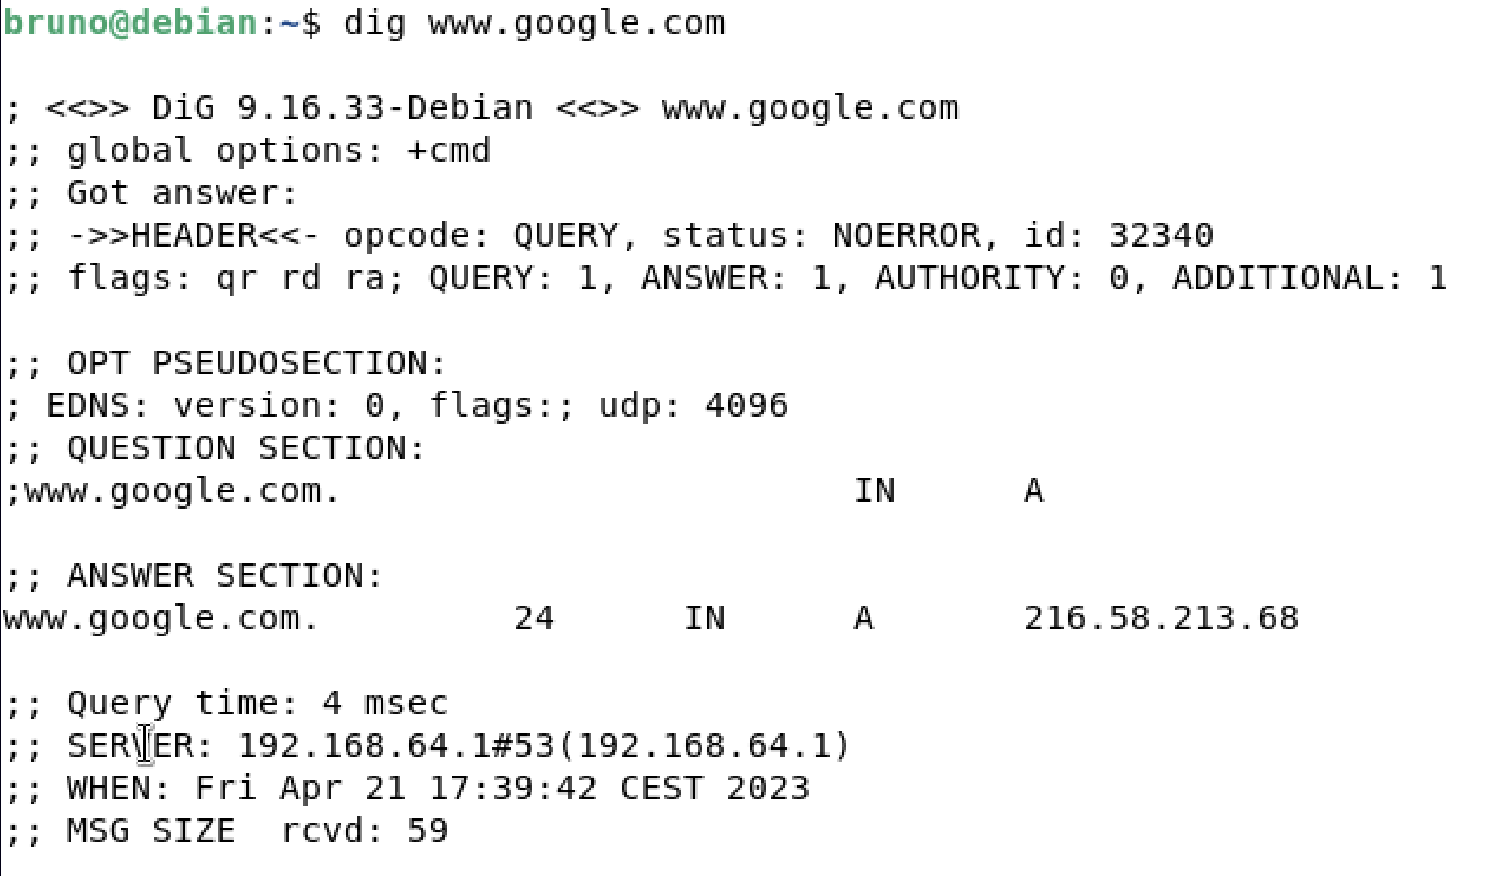
\includegraphics[scale=0.5]{images/dig-google.png}

\hbox{}

Now that our server is running we can visualize the packets that went trought it with Wireshark, the picture bellow shows the results from a ping to Google's website:

\hbox{}

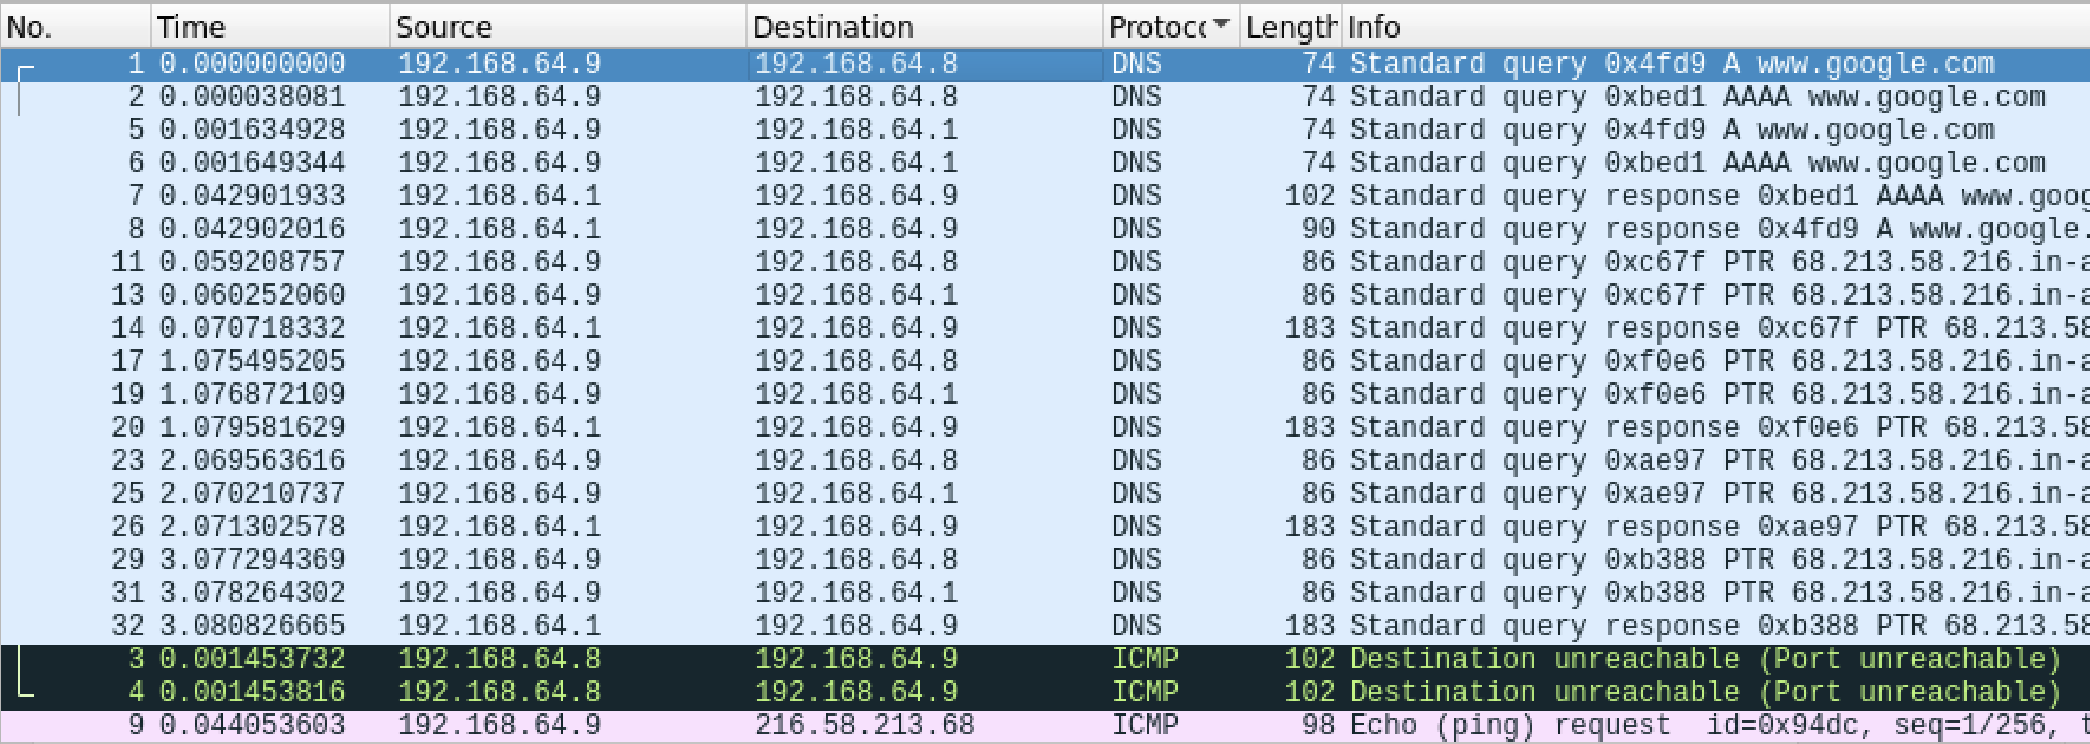
\includegraphics[scale=0.5]{images/ping-google.png}

\hbox{}

But a problem arises as the server is unreachable, this is caused by adding the following line of code requested at Step 1 from Task 2, ultimately causing the server to not be initialized.

\hbox{}

\definecolor{light-gray}{gray}{0.95}
\begin{lstlisting}[language=bash, frame=tlbr, framesep=6pt, backgroundcolor=\color{light-gray}]
  options{
    dump-file "/var/cache/bind/dump.db";
  };
\end{lstlisting}



\hbox{}

\pagebreak
\section{Bonus: Evaluation function improvement}

After implementing and running countless test to all algorithm proposed, we identified a serious problem with the evaluation function used in the project: It was the main piece holding our implementations back, and the perormance of our algorithms were suffering a lot because of it.

The default evaluation function implemented in the project is the \textit{\textbf{scoreEvaluationFunction}}. The evaluation function only takes into account the current score of the games. It gets the work done in some of the cases, but has two serious draw-backs: It doesn't take into account the number of food left in the maze, and it doesn't take into account the distance to the closest food. As a result, when the Pacman gets "isolated" in a part of the map without any food, it hasn't anything to maximize, and needs a ghost to approch in order to proceed the game.

To solve this problem, we sugest a new evaluation function, called \textit{\textbf{betterEvaluationFunction}}. It's implementation and functionallity is explained in the following section.

\subsection{The new evaluation function: betterEvaluationFunction}

The proposed evaluation function takes into account this two extra parameters (along with the score): \textit{the number of food pallets left} and \textit{the distance to the closest food}. The number of food pallets left encourages the Pacman to eat more pallets when stuck, and the distance to the closest food will prevent the Pacman of isolating itself in the maze.

the implementation is described in the following section.

\subsubsection{betterEvaluationFunction implementation}

To implement the new evaluation function, we created a new function in the code, as follows:

\begin{table}[!ht]
  \begin{lstlisting}[language=python, frame=tlbr, framesep=6pt, backgroundcolor=\color{light-gray}]
def betterEvaluationFunction(currentGameState):
  """
  Your extreme ghost-hunting, pellet-nabbing, food-gobbling, unstoppable
  evaluation function (question 8).

  DESCRIPTION: <write something here so we know what you did>
  """
  
  def closestFoodDistance(gameState):
    pacmanPosition = gameState.getPacmanPosition()
    foodList = gameState.getFood().asList()

    if len(foodList) == 0:
        return 0

    return min([manhattanDistance(pacmanPosition, food) for food in foodList])

  closestFood = closestFoodDistance(currentGameState)
  return currentGameState.getScore() - (10 * closestFood) \ 
    - (100 * currentGameState.getNumFood())
  \end{lstlisting}
  \caption{betterEvaluationFunction implementation}
\end{table}

For calculation the distance to the closest food, we used the the Manhattan Distance (implemented in the function itself), and the number of food is retrieved from the game state. They are multiplied by 10 and 100, respectively, in order to have a bigger impact in the final score, and subtracted from the current game score.

The results of our implementation is showed in the next section.

\subsubsection{betterEvaluationFunction tests}

To test the new \textit\textbf{{betterEvaluationFunction}}, we repeated the same tests executed before, now using the this new evaluation function instead of the old \textit\textbf{{scoreEvaluationFunction}}. We chose the  \textit\textbf{{Expectimax agent}} to run the tests. Its description and implementation can be found in Section~\ref{sec:expectimax}.
~\\
~\\
The result of the tests can be found in Table~\ref{tab:expectimax-better}.

~\\
\begin{table}[!ht]
  \begin{center}
    \begin{tabular}{||c||c|c|c|c||}
      \hline
      Depth & 2 & 3 & 4 \\
      \hline\hline
      Average &  1228.6 &  1340.15 &  1131.25 \\
      \hline\hline
      Best & 1724 & 1757 & 1743 \\
      \hline\hline
      Win Rate & 19/20 (0.95) & 20/20 (1.00) & 19/20 (0.95) \\
      \hline
    \end{tabular}
    \caption{Expectimax test results with betterEvaluationFunction}
    \label{tab:expectimax-better}
  \end{center}
\end{table}

Comparing both results of Tables~\ref{tab:expectimax} and~\ref{tab:expectimax-better}, it's possible to observe a huge gain in performance. By only altering the evaluation function, we were able to obtain way batter results, even reaching a Win Rate of 100\% in some test cases, and performing well in the cases with lower depths.

\pagebreak
\section{Conclusion}

This lab was essential on the understanding of the DNS server and the Firewall, by allowing us to create and configure them first-hand.
We were able to fully understand how to configure, run and realize attacks on a DNS server, we also got more used to the Linux environment as it was necessary to configure files and run commands on the bash terminal.
On top of that we also gained knowledge on the form of communication between the machines by using the Wireshark and Scapy tool to visualize the traffic on the network and the packets sent.

\end{document}